% oem_mapping.tex — grounded OpenEarthMap(OEM) <-> Biodiversity mapping SCHEMATIC.
%
% The picture form of Table 1. Two panels + a shared legend:
%   Panel A — hard argmax (Sankey): each OEM class -> its argmax Biodiversity class, arrow
%             coloured the TARGET Biodiversity colour, confidence % on the arrow. The three
%             rows that changed from the original name-based map (Bareland -> Seminatural,
%             Water -> Grassland, Agriculture -> Grassland) are drawn with a thick black
%             outline and a grey-italic "was -> ..." annotation. Teacher-pixel-share badges
%             on the OEM chips with >3% share.
%   Panel B — soft teacher distribution (9x6 heatmap): every cell prints P(GT student | teacher
%             OEM) x100, background = target student colour scaled by value; the per-row argmax
%             cell is bold-bordered to tie B back to A; cells <1% are blanked grey.
%
% ALL NUMBERS ARE GENERATED, NOT TRANSCRIBED:
%   scripts/figures/_gen_mapping_values.py loads artifacts/teacher_oem_gt_confusion.npz and prints
%   (a) the SOFT matrix row-normalised x100 (this is build_mapping_from_confusion(mode="B") x100),
%   (b) the per-row argmax (asserted == OEM_TO_STUDENT_PRETRAIN), and
%   (c) the teacher-pixel SHARE from the HARD array row-sums (Agriculture 66.8% etc.;
%       the SOFT array would give 63.4% for Agriculture and is NOT used for shares).
% The values embedded below are copied verbatim from that script's output.
%
% This is a SCHEMATIC (the value-scaled heatmap is a new schematic idiom), NOT a segmentation
% mask — do not reuse this rendering anywhere a real mask is drawn.
%
% House style (Sec 2.7): standalone + [T1]fontenc + tikz; >=Stealth; Computer Modern (no Times).
% Compile:  cd scripts/figures && pdflatex -interaction=nonstopmode -halt-on-error oem_mapping.tex
\documentclass[border=6pt]{standalone}
\usepackage[T1]{fontenc}
\usepackage{lmodern}
\usepackage{amsmath}
\usepackage{tikz}
\usetikzlibrary{positioning, arrows.meta, calc, fit, backgrounds}

% ── Student (Biodiversity) palette — geoseg/taxonomy.py STUDENT_PALETTE ──
\definecolor{cBack}{RGB}{0,0,0}
\definecolor{cForest}{RGB}{250,62,119}
\definecolor{cGrass}{RGB}{168,232,84}
\definecolor{cCrop}{RGB}{242,180,92}
\definecolor{cSettle}{RGB}{59,141,247}
\definecolor{cSemi}{RGB}{255,214,33}

% ── OEM 8-class palette (+ Unknown black) ──
\definecolor{oUnknown}{HTML}{000000}
\definecolor{oBare}{HTML}{800000}
\definecolor{oRange}{HTML}{00FF24}
\definecolor{oDev}{HTML}{949494}
\definecolor{oRoad}{HTML}{FFFFFF}
\definecolor{oTree}{HTML}{226126}
\definecolor{oWater}{HTML}{0045FF}
\definecolor{oAgri}{HTML}{4BB549}
\definecolor{oBuild}{HTML}{DE1F07}

\begin{document}
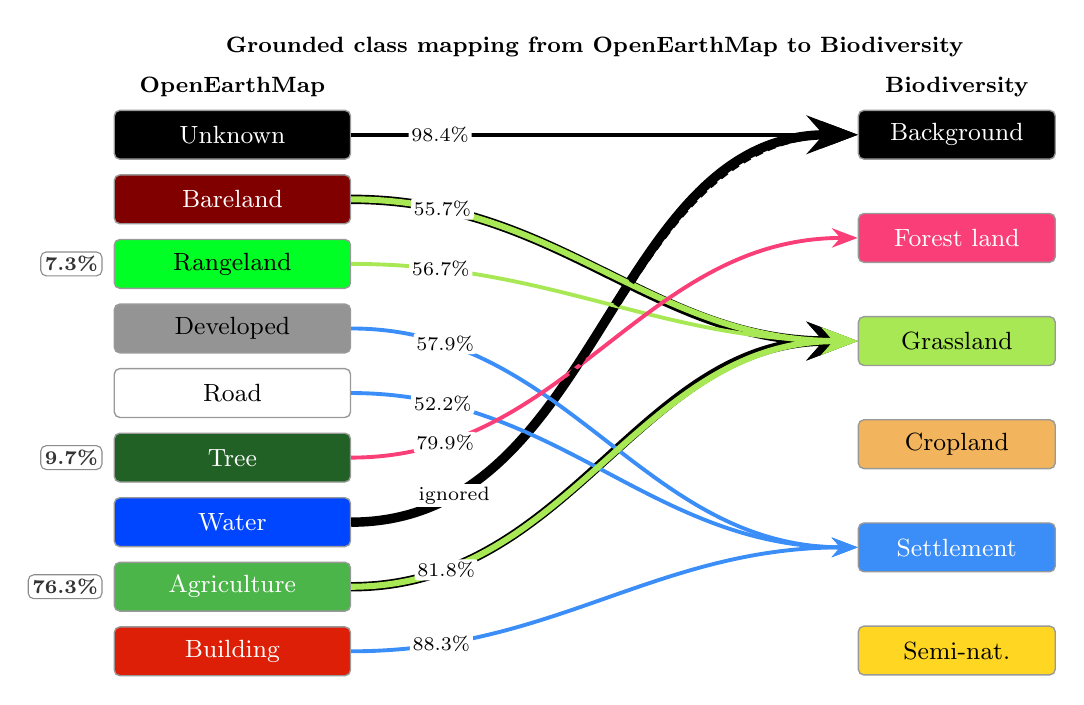
\begin{tikzpicture}[
  font=\small,
  >=Stealth,
  % OEM chip: fill = OEM colour, fixed size. White/black text set per chip.
  ochip/.style={
    rectangle, rounded corners=2pt, draw=black!40, line width=0.5pt,
    minimum width=3.0cm, minimum height=0.62cm, align=center, inner sep=2pt, font=\small
  },
  % student chip: fill = student colour.
  schip/.style={
    rectangle, rounded corners=2pt, draw=black!40, line width=0.5pt,
    minimum width=2.5cm, minimum height=0.62cm, align=center, inner sep=2pt, font=\small
  },
  % argmax arrow (normal): coloured the target student colour.
  arr/.style={->, line width=1.4pt},
  % argmax arrow for a CHANGED row: thicker + black halo behind.
  arrchg/.style={->, line width=2.2pt},
  conf/.style={fill=white, inner sep=1pt, font=\scriptsize, rounded corners=1pt},
  badge/.style={fill=white, draw=black!45, line width=0.4pt, rounded corners=2pt,
                inner sep=1.5pt, font=\scriptsize\bfseries, text=black!80},
  ann/.style={font=\scriptsize\itshape, text=black!65, inner sep=1pt},
  % Panel-B cell.
  cell/.style={rectangle, draw=black!18, line width=0.3pt,
               minimum width=1.02cm, minimum height=0.66cm, inner sep=0pt, font=\scriptsize},
  cellarg/.style={cell, draw=black, line width=1.3pt},
  hdr/.style={font=\footnotesize\bfseries, align=center},
]

% =====================================================================
% PANEL A — hard argmax (Sankey-style)
% =====================================================================
% OEM rows (top->bottom, OEM index order 0..8). y spacing 0.82cm.
\def\rowsep{0.82}
% (name, fill colour, white-text?, share-badge or empty)
% white-text chips: Unknown, Bareland, Tree, Water, Agriculture, Building, (Forest/Settlement on right)
\foreach \i/\nm/\col/\wt in {%
  0/Unknown/oUnknown/1,
  1/Bareland/oBare/1,
  2/Rangeland/oRange/0,
  3/Developed/oDev/0,
  4/Road/oRoad/0,
  5/Tree/oTree/1,
  6/Water/oWater/1,
  7/Agriculture/oAgri/1,
  8/Building/oBuild/1%
}{
  \pgfmathsetmacro{\yy}{-\i*\rowsep}
  \ifnum\wt=1
    \node[ochip, fill=\col, text=white] (oem\i) at (0,\yy) {\nm};
  \else
    \node[ochip, fill=\col, text=black] (oem\i) at (0,\yy) {\nm};
  \fi
}

% Teacher-pixel SHARE badges (HARD array; _gen_mapping_values.py), share > 3%.
% REGROUNDED 2026-07-26 on the spatially blocked training split; refreshed here 2026-07-28.
%   Unknown 1.7, Bareland 0.4, Rangeland 7.3, Developed 0.9, Road 1.0, Tree 9.7, Water 1.8,
%   Agriculture 76.3, Building 1.0.  Only three now clear the 3% rule, so the Unknown and Water
%   badges are dropped rather than shown below their own threshold.
% Placed immediately LEFT of each chip, vertically centred on its OWN row, so the share is
% unambiguously tied to its OEM class (not the chip above) and never hits the arrow start (right side).
\node[badge, anchor=east] at ([xshift=-4pt]oem2.west) {7.3\%};
\node[badge, anchor=east] at ([xshift=-4pt]oem5.west) {9.7\%};
\node[badge, anchor=east, font=\scriptsize\bfseries] at ([xshift=-4pt]oem7.west) {76.3\%};

% The three rows whose grounded target differs from naive name-based matching (Bareland,
% Water, Agriculture) are marked by the thick black arrow outline below; the cryptic
% "was -> ..." left-margin annotations were removed (the bold arrow + key carry this).

% Student chips (right column). Wider horizontal channel (x=9.2) keeps the curves shallow.
% white-text: Background, Forest, Settlement. black-text: Grassland, Cropland, Seminatural.
\def\stx{9.2}
\foreach \j/\nm/\col/\wt/\yy in {%
  0/Background/cBack/1/0.0,
  1/{Forest land}/cForest/1/-1.31,
  2/Grassland/cGrass/0/-2.62,
  3/Cropland/cCrop/0/-3.93,
  4/Settlement/cSettle/1/-5.24,
  5/{Semi-nat.}/cSemi/0/-6.55%
}{
  \ifnum\wt=1
    \node[schip, fill=\col, text=white] (st\j) at (\stx,\yy) {\nm};
  \else
    \node[schip, fill=\col, text=black] (st\j) at (\stx,\yy) {\nm};
  \fi
}

% --- argmax arrows: OEM i -> student argmax, coloured the TARGET student colour. ---
% (oem, student-target, target-colour, conf%, changed?)
% REFRESHED 2026-07-28 from _gen_mapping_values.py on the regrounded teacher confusion.
%   Unknown->Background 98.4 ; Bareland->Grass 55.7 CHG ; Rangeland->Grass 56.7 ;
%   Developed->Settle 57.9 ; Road->Settle 52.2 ; Tree->Forest 79.9 ;
%   Water->IGNORED (see below) ; Agriculture->Grass 81.8 CHG ; Building->Settle 88.3.
% Bareland moved from Semi-natural to Grassland in the 2026-07-26 regrounding, so NO OEM class now
% maps to Semi-natural or to Cropland.
% Black halo first for the changed rows, then the coloured arrow on top.
\foreach \oi/\sj in {1/2, 6/0, 7/2}{
  \draw[->, line width=3.4pt, black, rounded corners]
    (oem\oi.east) to[out=0,in=180] (st\sj.west);
}
% Confidence labels are anchored NEAR THE SOURCE (pos=0.16) so each sits beside its own OEM
% row and they fan out vertically instead of stacking at the convergence point.
\foreach \oi/\sj/\col/\cf/\chg in {%
  0/0/cBack/98.4/0,
  1/2/cGrass/55.7/1,
  2/2/cGrass/56.7/0,
  3/4/cSettle/57.9/0,
  4/4/cSettle/52.2/0,
  5/1/cForest/79.9/0,
  7/2/cGrass/81.8/1,
  8/4/cSettle/88.3/0%
}{
  \ifnum\chg=1
    \draw[arrchg, \col, rounded corners] (oem\oi.east) to[out=0,in=180]
      node[conf, pos=0.16, text=black]{\cf\%} (st\sj.west);
  \else
    \draw[arr, \col] (oem\oi.east) to[out=0,in=180]
      node[conf, pos=0.16, text=black]{\cf\%} (st\sj.west);
  \fi
}

% Water is drawn separately because it is the one row where the shipped mapping is NOT the argmax of
% the teacher confusion. The target taxonomy has no water class, so OEM Water is mapped to Background
% and IGNORED during pre-training (geoseg/taxonomy.py). Its argmax would have been Grassland at
% 75.2%, and drawing that arrow -- as this figure did until 2026-07-28 -- shows a mapping the model
% was never trained with. A confidence percentage would be meaningless here, so the label says what
% the row actually does.
\draw[arrchg, cBack, rounded corners, densely dashed] (oem6.east) to[out=0,in=180]
  node[conf, pos=0.16, text=black]{ignored} (st0.west);

% Panel-A title
\node[hdr, anchor=south] at ($(oem0.north)!0.5!(st0.north)+(0,0.55)$)
  {Grounded class mapping from OpenEarthMap to Biodiversity};
\node[font=\footnotesize\bfseries, anchor=south] at ([yshift=1pt]oem0.north) {OpenEarthMap};
\node[font=\footnotesize\bfseries, anchor=south] at ([yshift=1pt]st0.north) {Biodiversity};


% =====================================================================
% No in-figure legend or key: every class is already a named, colour-filled chip in both
% panels, and the encoding (arrow/cell colour = target class; bold outline = differs from
% name-based matching; left badges = teacher-pixel share) belongs in the manuscript caption.
% =====================================================================

\end{tikzpicture}
\end{document}
